\documentclass{article}

%\usepackage{preamble}
%\usepackage{draftwatermark}
%	\SetWatermarkText{EXAMPLE}
%	\SetWatermarkScale{5}

%FOR FUNKY TITLE PAGE
% \usepackage{./files/titlepreamble}
	\usepackage{xstring,ifthen}			% for coding and boolean in "titlepreamble.sty"
	\usepackage{datetime}				% for accurate dates and times

%PAGE FORMATTING
  %FORMAT
  	\usepackage{microtype}
	\usepackage[colorlinks=true]{hyperref}	% funky bright links
		\hypersetup{ %
			urlcolor=	blue,		%default: magenta
			linkcolor=	red,		%default: red
			anchorcolor=black,		%default: black
			citecolor=	green,		%default: green
			filecolor=	cyan,		%default: cyan
			menucolor=	red,		%default: red
			runcolor=	cyan,		%default: cyan
			allcolors=	blue,		%will replace all previous
		}
	\usepackage{sectsty}					% section heading formatting
		\allsectionsfont{\normalfont\sffamily\bfseries}			% ALL HEADINGS: bold, sans-serif
		\chapterfont{\flushright\normalfont\sffamily\bfseries}	% All CHAPTERS: (above +) right-aligned
  %FONT
	\renewcommand{\familydefault}{\sfdefault}	% FONT STYLE FOR ENTIRE DOCUMENT
  %SPACING
	\usepackage{fullpage}					% wide margins
	\usepackage[parfill]{parskip}			% paragraph spacing
  %LAYOUT
	\usepackage[bottom]{footmisc}			% make footnotes appear at page bottom
  %SI UNITS
  	\usepackage{siunitx}					% provides SI units in appropriate formatting
		\sisetup{separate-uncertainty=true}	% allows plus-minus errors
		\newcommand{\cm}{\centi\metre}
		\newcommand{\mm}{\milli\metre}
		\newcommand{\mT}{\milli\tesla}
	
%BOOK FORMATTING
\usepackage{fancyhdr}						% nice header format
	\fancyhead[RO, LE]{\textbsf{\thepage}}		% page numbers, on both odd and even
	\fancyhead[LO]{\textbsf{\leftmark}}			% chapter headings
	\fancyhead[RE]{\textbsf{\rightmark}}		% section headings
%\renewcommand{\chaptername}{Lecture}		% change "Chapter" to "Lecture"

%AMS PACKAGES
\usepackage{amsmath}					% better equations
\usepackage{amssymb}					% more symbols

%TABLES AND FIGURES
\usepackage{float}						% allows floats (really bad)
\usepackage{caption}					% options for figure captions
	\captionsetup{ %
		labelfont=bf,					% bold caption title
		font=small,						% small caption text
		}
\usepackage{wrapfig}					% really bad package for text wraps
  %TABLES				
	\usepackage{tabularx}					% allows more adaptible tables (also really bad)
  %GRAPHICS
	\usepackage{graphicx} 					% insertion of figures
	\usepackage{epstopdf}					% vector graphics
		\DeclareGraphicsExtensions{.eps, .pdf, .gif}

%BIBLIOGRAPHY
\usepackage[numbers]{natbib}
%	\bibliographystyle{apalike}
	\bibliographystyle{unsrtnat}
	\newcommand{\biblocation}{../master_bibliography}	% causes scoping failure (default:	"./files/bibliography")
	\newcommand{\printbib}{ %
		\IfStrEq{\biblocation}{}{ %
			\bibliography{../master_bibliography}
			}{ %
			\bibliography{\biblocation}
			}
		}
	
%OTHER PACKAGES
\usepackage{color}						% able to colour anything and use colour boxes
\usepackage{pst-node}					% easy relative alignment
	\usepackage{pstricks}
\usepackage{tikz}
	\usetikzlibrary{tikzmark}

% vertical equals
\newcommand\rotateequal[1]{%
  \ifmmode
    \underset{#1}{\rotatebox{90}{$=$}}%
  \fi
}

\newenvironment{hang}
	{\list{}{%
		\rightskip 	1cm
		\parindent	1cm
		\itemindent-1cm
	}\item[]}
	{\endlist}
	
%FORMATTING OPTIONS
  %SANS-SERIF BOLD	[~bsf]
	\newcommand{\mathbsf}[1]{\mathbf{\mathsf{#1}}}
	\newcommand{\textbsf}[1]{\textbf{\textsf{#1}}}
  %QUOTATIONS
  	\usepackage [autostyle, english = american]{csquotes}
  		\MakeOuterQuote{"}					% allows ""
  	\renewcommand{\quote}[1]{``#1''}		% allows "" -> \quote{}
  %SUPER-/SUB-SCRIPT
	\newcommand{\super}[1]{\textsuperscript{#1}}
	\newcommand{\sub}[1]{\textsubscript{#1}}

%SHORTHAND
  %LATIN SHORTHAND
	\newcommand{\eg}{\emph{e.g.}\,}
	\newcommand{\ie}{\emph{i.e.}\,} 
  %OTHER SHORTHAND
	\newcommand{\Schr}{Schr{\"o}dinger\ }
	\newcommand{\dd}{\mathrm{d}}

%NOTATION
  %VECTOR NOTATION
	\renewcommand{\v}[1]{\mathbf{#1}}			% for vectors
  %BRA-KET NOTATION
	\renewcommand{\b}[1]{\big\langle {#1} \big|}
	\renewcommand{\k}[1]{\big| {#1} \big\rangle}
	\newcommand{\bk}[2]{\big\langle {#1} \big| {#2} \big\rangle}
	\newcommand{\expct}[1]{\big\langle {#1} \big\rangle}
	\newcommand{\pamp}[1]{\big|#1\big|^2}
  %SET NOTATION
	\newcommand{\set}[1]{\left\{#1\right\}}
	
%SYMBOLS
	\newcommand{\nablab}{\boldsymbol{\nabla}}	% vector del, 	"NABLA Bold"
	\newcommand{\epsn}{\epsilon_0}				% epsilon_0,	"EpSilon Nought"

%COLORS
	\definecolor{darkgray}		{rgb}{0.2,0.2,0.2}
	\definecolor{gray}		{rgb}{0.5,0.5,0.5}
	\definecolor{lightgray}	{rgb}{0.8,0.8,0.8}
	\definecolor{lightergray}	{rgb}{0.95,0.95,0.95}
	\definecolor{lighterblue}	{rgb}{0.95,0.95,1.0}	
	\definecolor{darkgreen}		{rgb}{0.0,0.5,0.0}
	
\newcommand{\note}[1]{\colorbox{lightgray}{[#1]}}
\newcommand{\tab}{\hspace{2em}}

\newcommand{\sampleA}{$ \left[\text{Fe}(\text{Htrz})_2(\text{trz})\right](\text{BF}_4) $}
\usepackage{setspace}
\doublespacing
\usepackage{multicol}
\newcommand{\labtools}{SCO \texttt{LabTools}}
%\usepackage{minted}	% too complicated

\newcommand{\cd}[1]{%
	\colorbox{lightergray}{%
		\begin{minipage}{\linewidth}
			\texttt{#1}
		\end{minipage}
	}
}%\colorbox{lightergray}{\texttt{#1}}}	% code

\newcommand{\gencd}[1]{\texttt{\textit{\textcolor{darkgray}{<#1>}}}}	% general code
\newcommand{\user}{\gencd{user}}
\renewcommand{\root}{\gencd{root}}
\newcommand{\flags}{\gencd{flags}}
\newcommand{\inpath}{\gencd{input path}}
\newcommand{\outpath}{\gencd{output path}}

%DOCUMENT INFO
\title{PH700 Project Software User Guide\\
		\textbf{SCO \texttt{LabTools} Package}}
\author{Harry Smith\thanks{hs339@kent.ac.uk}\ \thanks{Under supervision of Helena Shepherd.}}
\date{\today}

\begin{document}

%\maketitle

\tableofcontents

\pagebreak
\section{Introduction}
\labtools{} is developed using the Python 3 language. It is a comprehensive toolkit for SCO research, which provides programs to plot graphs from common measurement methods: namely, SQUID magnetometry, Raman spectroscopy and reflectometry.

The intention of this software package is to be as user-friendly as practically possible. Unfortunately, no time allowed for introduction of a guided user interface (GUI) so the code will have to be run from the terminal; to compensate, this manual will be comprehensive. Please refer to this manual as your first port of call for help.

\section{Installation}
\subsection{Installing Python 3 (Anaconda 3)}
\labtools{} requires that the Python 3 have access to both scientific \& numeric modules and elements of the Python imaging library (PIL): the Anaconda 3 distribution of Python comes as standard with all of these required modules.

\begin{center}
\colorbox{lighterblue}{%
	\href{https://www.continuum.io/downloads}{Download Anaconda 3 from \texttt{https://www.continuum.io/downloads}}
}
\end{center}%

This will probably install Anaconda 3 to the \texttt{C://Users/\user{}/Anaconda3/} directory.

% WRITE MORE ABOUT INSTALLATION

\subsection{Installing additional dependencies}

Hopefully, Anaconda should contain all the dependencies (\ie{} packages, modules) we need. Just to be sure, we can explicitly install requirements using pip (pip should be installed with Python). We can do this using the requirements.txt file placed in the SCOLabTools project folder by running the following at the terminal line:

\cd{%
\begin{hang}
>>	pip install -r requirements.txt
\end{hang}%
}

\pagebreak
\section{Running}
\subsection{Running programs}

Codes must be run from the command line in the terminal. For Windows users this means using \textit{Command Prompt}.

\textbf{Point to the interpreter.} Load up the terminal and do the following:

\begin{enumerate}
\item	Locate the interpreter.
\item[]	We must tell the terminal \textit{where} our interpreter is\footnote{We can instead include Python 3 to our PATH variable---meaning we can call our Anaconda 3 distribution using the simple command \texttt{python}---but this is more complicated than it needs to be so I'll leave it out. Google it if you want to do this but be careful you don't accidentally default to Python 2 because the code won't run.}. 	The interpreter will be reading the code and translating it from human readable Python code to a list of binary instructions which the computer can understand.
 
\begin{itemize}
\item We will be using Python 3 to interpret, so we need to include the path of the Python distribution we want to use, which will be located in the Anaconda 3 directory (probably \texttt{C://Users/\user{}/Anaconda3}, where \user{} is the name of the user who installed Anaconda.) Try looking through the directory structure for the named '\texttt{Anaconda3}' if you're unsure which user has installed Anaconda 3.
\item	Inside the \texttt{Anaconda3} directory there should be a file named '\texttt{python.exe}'. This is our interpreter.
\end{itemize}

\item 	Copy interpreter file path. 
\begin{itemize}
\item[]	On Windows, to get the path to the \texttt{python.exe} file, hold shift and right-click. Select 'Copy as path' from the drop-down menu: this will save the path to your clipboard.
\end{itemize}

\item	Now go back to your terminal window, right click and select 'Paste' from the drop-down menu. 
\begin{itemize}
\item[]	Note that the keyboard shortcut '\texttt{Ctrl + v}' does not work.
\end{itemize}

\end{enumerate}

In your terminal window you should now have\footnote{The "\texttt{>>}" signifies that we're talking about the command line input. You do not need to include this when you write into the terminal. Think of it like a bullet point in a list.}:

\cd{%
\begin{hang}
>>	C://\gencd{path to Anaconda}/Anaconda3/python.exe
\end{hang}%
}

\textbf{Point to the program.} Now we can locate the program we want to run.

\begin{enumerate}
	\item	Locate program code file in directory structure. This will have the extension '\texttt{.py}' or '\texttt{.pyc}'.
	\item	Copy code file path. Windows: \texttt{Ctrl} + right-click, 'Copy as path'.
	\item	Paste code file path into terminal next to interpreter path.
\end{enumerate}

In your terminal window you should now have:

\cd{%
\begin{hang}
>>	C://\gencd{path to Anaconda}/Anaconda3/python.exe \tab C://\gencd{path to program}/\gencd{program name}.py
\end{hang}%
}

At this point, one must include compulsory command line arguments after the program or optional command line arguments after flags. \labtools{} does not use any compulsory arguments but here is the general structure:

\cd{%
\begin{hang}
>>	C://\gencd{path to Anaconda}/Anaconda3/python.exe \tab C://\gencd{path to program}/\gencd{program name}.py \gencd{compulsory args} \gencd{optional flags}
\end{hang}%
}

More detail is provided in the next section.

\subsection{Using flags}\label{ssec:running:flags}
Flags are optional command line arguments which follow the calling of a code. They are called using a hyphen '\texttt{-}' or double-hyphen '\texttt{--}' proceeded by an identifying word or letter, the \gencd{flag id}. The argument of the flag, the \gencd{flag arg}, is then given after a blank space.

In general:

\cd{%
\begin{hang}
>>	\textcolor{red}{\textit{<interpreter>}.exe} \textcolor{darkgreen}{\textit{<program>.py}} \textcolor{blue}{-\textit{<flag1 id>} \textit{<flag1 arg>}} \textcolor{magenta}{-\textit{<flag2 id>} \textit{<flag2 arg>}} $ \cdots $
\end{hang}%
}

Examples of running using flags follow:

\begin{itemize}
\item[(1)]	%
	\cd{%
	\begin{hang}
	>>	D://Interpreters/Anaconda3/python.exe C://Python/Projects/io\_program.py --input C://Documents/Path/to/input/dir/ --output F://Documents/Path/to/output/dir/
	\vspace{1em}%
	\end{hang}%
	}
\item[] This is a standard input/output (IO) example. Here, the user specifies their interpreter to be in their chosen interpreters depository on their \texttt{D} drive, '\texttt{D://Interpreters/}, where they use Anaconda 3's Python interpreter to run the program '\texttt{io\_program.py}'. The flags \texttt{--input} and \texttt{--output} intuitively specify the paths to the relevant directories.
%
\item[(2)]	%
	\cd{%
	\begin{hang}
	>>	C://Users/User1/Anaconda3/python.exe C://MyPythonCodes/python\_code.py -p C://Documents/Path/to/input/file.in --diagonalize True
	\vspace{1em}%
	\end{hang}%
	}
\item[]	This example calls the Anaconda 3 Python interpreter '\texttt{python.exe}' from the default location and asks it to interpret the program code '\texttt{python\_code.py}' from this user's code depository directory, '\texttt{C://MyPythonCodes/}' using the optional flags, '\texttt{-p}' and '\texttt{--diagonalize}'. Evidently, '\texttt{-p}' expects a file path; '\texttt{--diagonalize}' expects a Boolean (or logical) specification.
\end{itemize}


\pagebreak
\section{Creating External Files}
Many of programs require external files to provide information in order to run effectively. The most common are as follows:

\begin{table}[H]
	\begin{center}
		\begin{tabular}{l l l l}
			\hline
			\textbf{File}	&	\textbf{Description}	&	\textbf{Compulsory?} & \textbf{Notes}\\
	%		\hline
			\texttt{times.dat}	& Image creation times file	&	No	&	Required for intuitive temperature.	\\
			\texttt{curve.dat}	& Curve profile file	&	No	&	Required for intuitive temperature.	\\
			\texttt{roi.dat}	& Region of Interest (ROI) file	&	No	&	\\
			\texttt{config.yaml}	& Configuration file	&	No	&	\\
			\hline
		\end{tabular}
	\end{center}
	\caption[External files summary.]{\label{tab:ext_files:overview}%
		Summary of common external files used by codes in \labtools{}.%
	}
\end{table}

\subsection{Creating \texttt{.dat} and \texttt{.yaml} files by hand}



\subsection{Image creation times file, \texttt{times.dat}}
The \texttt{times.dat} file must be created using the \texttt{time.py} program.

\subsection{Curve profile file, \texttt{curve.dat}}\label{ssec:ext_files:curve}
The \texttt{curve.dat} file may be produced by hand; it does not require the use of additional software to create the file. 

\subsubsection{General format}
For a curve profile of $ n $ elements, the \texttt{curve.dat} file has the following general formulation:

\cd{%
\begin{tabular}{lll}
rate$ _1 $ &	limit$ _1 $ &	time$ _1 $ \\
rate$ _2 $ & 	limit$ _2 $ &	time$ _2 $ \\
$ \vdots $ &	$ \vdots $ &	$ \vdots $ \\
rate$ _n $ &	limit$ _n $ &	time$ _n $ \\
\end{tabular}
\vspace{1em}%
}

Notice here that every element on each row is separated by a \textit{tab}.

Rates are in degrees Celsius per minute, $ \si{\degreeCelsius\per\minute} $; limits are in degrees Celsius, $ \si{\degreeCelsius} $; and wait times are in minutes, $ \si{\minute} $. This is almost analogous to the process of inputting a temperature curve profile into the Linkam temperature stage, with the exception of the time. If you have a time $ t $ in seconds and need to convert to minutes, use the conversion formula

\begin{equation}\label{eq:sec_to_min_conv}
	t_\text{minutes} = 0.0167\,t_\text{seconds}.
\end{equation}

\subsubsection{Examples}
\begin{itemize}
\item[(1)]%
\cd{
\begin{tabular}{lll}
50.00 &	25.0 &	1.00 \\
10.00 &	70.0 &	5.00 \\
10.00 &	130.0 &	5.00 \\
10.00 &	160.0 &	5.00 \\
10.00 &	130.0 &	5.00 \\
10.00 &	70.0 &	5.00 \\
10.00 &	25.0 &	5.00 \\
10.00 &	70.0 &	5.00 \\
10.00 &	130.0 &	5.00 \\
10.00 &	160.0 &	5.00 \\
10.00 &	130.0 &	5.00 \\
10.00 &	70.0 &	5.00 \\
10.00 &	25.0 &	5.00 \\
10.00 &	70.0 &	5.00 \\
10.00 &	130.0 &	5.00 \\
10.00 &	160.0 &	5.00 \\
10.00 &	130.0 &	5.00 \\
10.00 &	70.0 &	5.00 \\
10.00 &	25.0 &	60.00 \\
\end{tabular}
}
\item[] This example is a temperature curve at \SI{10}{\degreeCelsius\per\minute} with a wait time of \SI{5}{\minute} between every section of the curve: it produces the curve shown in figure \ref{fig:ext_files:curve:ex1}.\\
\begin{figure}[H]
\centering
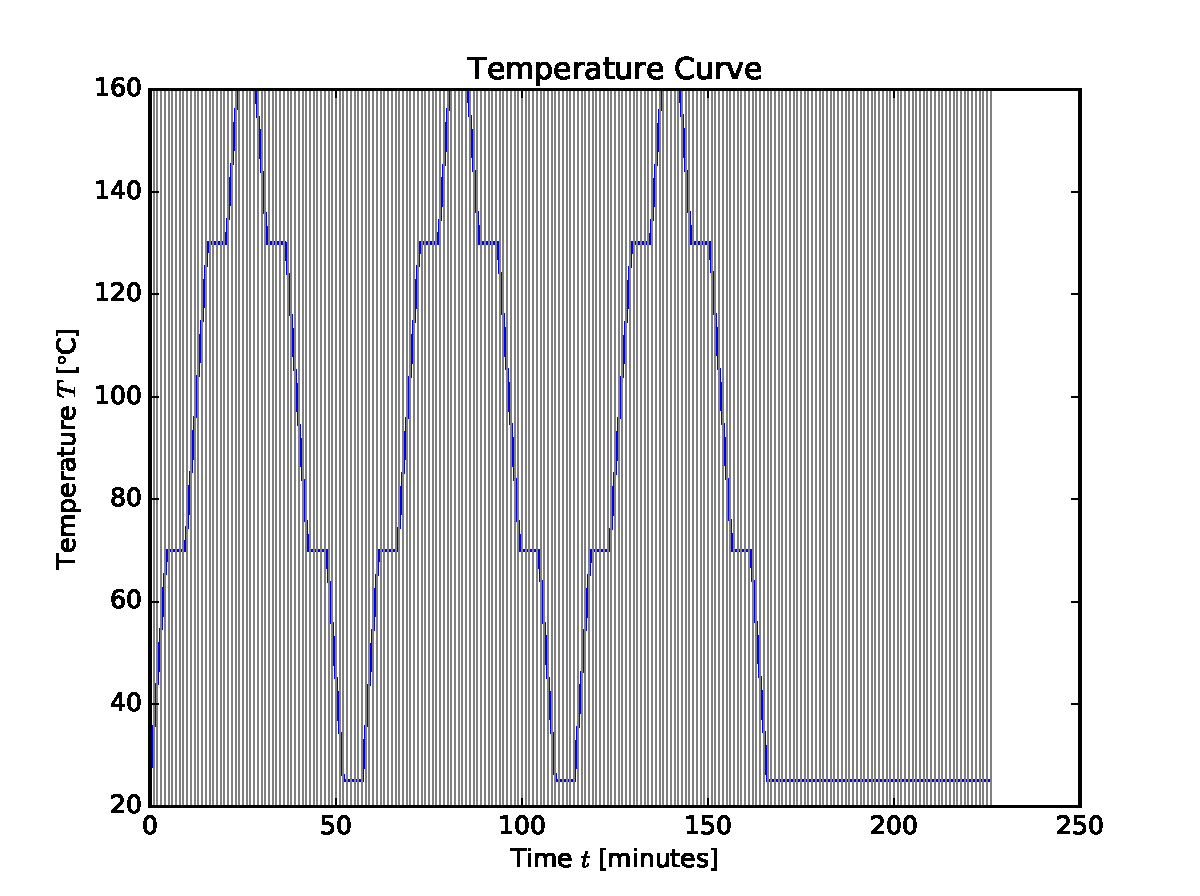
\includegraphics[width=0.7\linewidth]{./files/Temp_curve_ex_1-pdf}
\caption{Temperature curve for the profile in example (1).}
\label{fig:ext_files:curve:ex1}
\end{figure}
\end{itemize}

\subsection{Region of Interest (ROI) file, \texttt{roi.dat}}
The \texttt{roi.dat} file specifies the region of interest within the image. It may be produced by hand.

\subsubsection{General format}

\cd{%
\begin{tabular}{lll}
$ x_0 $	&	$ y_0 $ &	window\_width
\end{tabular}
}

Here, $ x_0 $ and $ y_0 $ specify the initial $ x $ and $ y $ co-ordinates of the ROI, window\_width specifies the window width, such that the ROI will have the top-left co-ordinate ($ x_0 $, $ y_0 $) and the bottom-right ($ x_0 + \text{window\_width} $, $ y_0 + \text{window\_width} $).


\subsection{Configuration files, \texttt{config.yaml}}
For most of the codes, configuration files are depreciated. Some still use them, however.

It is important to note that \textit{Boolean operators are entirely lower case} in configuration files due to the conventions of the YAML. Thus, \texttt{\textit{TRUE}} is designated '\texttt{true}' and \texttt{\textit{FALSE}} is designated '\texttt{false}'.


\subsubsection{Config files for \texttt{plot.py}}

\begin{minipage}{\linewidth}
\textbf{Example config file}

\cd{\\%
\textit{title:} Rate-dependency of Hysteresis\\
\textit{xlabel:} Ramping rate \$ \textbackslash dot{T} \$ [K/min]\\
\textit{ylabel:} Thermal hysteresis width \$ \textbackslash Delta T \$ [K]\\
\\
\textit{format}: o\\
\textit{grid}: false\\
\\
\textit{outname}: graph\_rate\_Dtemp\\
\textit{outexts}: [.png, .pdf, .svg]\\
\\
\textit{fitline}: true\\
\textit{a}: 1.5\\
\textit{b}: 36.125\\
\textit{linerange}: [-1, 12]\\
\\
\textit{errorprovided}: true\\
\textit{biglabels}: true\\
}
\end{minipage}


\textbf{Line fitting, \texttt{\textit{fitline}}}

Uses the equation

\begin{equation}
	y = a\,x + b.
\end{equation}

\textbf{Exponential fitting, \texttt{\textit{fitexp}}}

Uses the equation

\begin{equation}
	y = a\,e^{b\,x}.
\end{equation}

\textbf{Additional notes}
\begin{itemize}
\item 	If \colorbox{lightergray}{\texttt{\textit{errrorprovided}: true}}, the input \texttt{data.dat} file must be of the following general form:
\item[] \cd{
				\begin{tabular}{ccc}
					$ x_1 $ & $ y_1 $ & $ \Delta y_1 $ \\
					$ x_2 $ & $ y_2 $ & $ \Delta y_2 $ \\
					$ \vdots $ & $ \vdots $ & $ \vdots $ \\
					$ x_n $ & $ y_n $ & $ \Delta y_n $ \\
				\end{tabular}
				}
\item	For general advice on using YAML files, see the guide provided by \textit{Robot Has No Heart} here:
\item[] \tab \href{https://rhnh.net/2011/01/31/yaml-tutorial/}{https://rhnh.net/2011/01/31/yaml-tutorial/}\footnote{Date accessed: 2017-02-28.}.
\item	For general advice on appropriate \texttt{matplotlib} graphing \texttt{format}s, see the \texttt{matplotlib} documentation.
\end{itemize}

\pagebreak
\section{Reflectivity, \texttt{reflectivity.py}}
This section refers specifically to the program located at \texttt{\root{}/SCOLabTools/reflectivity.py}. The program can be called using the following general form:

\cd{%
\begin{hang}
	>>	\gencd{path to Anaconda}/Anaconda3/python.exe \tab	\root{}/SCOLabTools/reflectivity.py \tab	\flags{}
	\vspace{1em}%
\end{hang}%
}

The code will run the following processes:

\begin{enumerate}
	\item	Obtain input directory. (required)
	\item[]	%
		{One has the choice to provide an input directory at the command line or during running. The flags are provided in table \ref{tab:reflectivity:flags}. For more information on using flags, see section \ref{ssec:running:flags}.
		
		\begin{table}[H]
			\begin{center}
				\begin{tabular}{l l l}
					\hline
					\textbf{Flag}	&	\textbf{Description}	&	\textbf{Required?}\\
			%		\hline
					\texttt{-i} or \texttt{--input}	& Input directory path	&	No	\\
					\texttt{-o} or \texttt{--output}	& Output directory path	&	No	\\
					\hline
				\end{tabular}
			\end{center}
			\caption[Reflectivity flags.]{\label{tab:reflectivity:flags}%
				Flags for optional command line arguments in \texttt{reflectivity.py}.%
			}
		\end{table}
		
		Notice that the flags are not required to run the code. If the input directory is excluded from the command line arguments the program will simply ask the user to provide an input directory via the terminal.
		
		\cd{%
		\begin{hang}%
		>> C://Users/\user/Anaconda3/python.exe C://Users/\user/.../SCOLabTools/reflectivity.py\\
		Running `reflectivity.py`.\\
		Please provide an input path: $ \blacksquare $
		\vspace{1em}%
		\end{hang}%
		}
		}
	\item	Reads and processes optional configuration files from input directory.
	\begin{enumerate}
		\item 	Reads ROI file, \texttt{\gencd{input dir}/output/roi.dat}.
		\item	Reads temperature curve profile file, \texttt{\gencd{input dir}/output/curve.dat}.
		\item	Reads file creation times file\footnote{File creation times file \textbf{must} be produced using the \textit{original} images, not copies. Please see section \ref{ssec:misc:times} for more information on running the \texttt{times.py} code to produce a \texttt{times.dat} file.}, \texttt{\gencd{input dir}/output/times.dat}.
		\item	Reads config file, \texttt{\gencd{input dir}/config.yaml}. Note this is depreciated in the most recent versions of this code but can still provide useful input.
	\end{enumerate}
	\item	Produces a function describing the temperature curve (uses \texttt{curve.py}.)
	\item	Reads and processes images from input directory.
	\begin{enumerate}
		\item 	Reads each image, indexed $ i $.
		\item	Crops $ i $\super{th} image to ROI.
		\item	Compresses cropped $ i $\super{th} image.
		\item	Extracts color (RGB) data for each pixel in cropped $ i $\super{th} image and calculates mean. Also calculates grayscale (k) intensity.
	\end{enumerate}
	\item	Plots and outputs graphs.
	\item[]	Graphs will be saved to output directory under the names '\texttt{graph.\gencd{ext}}', where \gencd{ext} $ \in $ \{.png, .pdf, .svg\} by default.
	\item[]	Graph axes are intuitively plotted: if temperature data is available then intensity \textit{vs.} temperature will be plotted, else intensity \textit{vs.} image number (can be related to time) will be plotted.
	\item[]	Hysteresis loops will be automatically split into individual loops with different colours for each loop.
\end{enumerate}

\subsection{Example of output}

\begin{figure}[H]
\centering
\includegraphics[width=0.7\linewidth]{C:/Users/Harry/Documents/PH700/Reflectivity/Images/Test_11/output/graph_k}
\caption{SCO transition curve using reflectometry. Plotted using default output option of \texttt{reflectivity.py}.}
\label{fig:graph_k}
\end{figure}


\pagebreak
\section{Raman, \texttt{raman.py}}

This section refers specifically to the program located at \texttt{\root{}/SCOLabTools/raman.py}. The program can be called using the following general form:

\cd{%
\begin{hang}
	>>	\gencd{path to Anaconda}/Anaconda3/python.exe \tab	\root{}/SCOLabTools/raman.py \tab	\flags{}
	\vspace{1em}%
\end{hang}%
}

The code will run the following processes:

\begin{enumerate}
	\item	Obtain input directory. (required)
	\item[]	%
		{One has the choice to provide an input directory at the command line or during running. The flags are provided in table \ref{tab:raman:flags}. For more information on using flags, see section \ref{ssec:running:flags}.
		
		\begin{table}[H]
			\begin{center}
				\begin{tabular}{l l l}
					\hline
					\textbf{Flag}	&	\textbf{Description}	&	\textbf{Required?}\\
			%		\hline
					\texttt{-i} or \texttt{--input}		& Input directory path	&	No	\\
					\texttt{-o} or \texttt{--output}	& Output directory path	&	No	\\
					\hline
				\end{tabular}
			\end{center}
			\caption[Raman flags.]{\label{tab:raman:flags}%
				Flags for optional command line arguments in \texttt{raman.py}.%
			}
		\end{table}
		
		Notice that the flags are not required to run the code. If the input directory is excluded from the command line arguments the program will simply ask the user to provide an input directory via the terminal.
		}
	%
	\item	Read data from input directory.
	\item	Normalise the data between 0 and 1 to minimum and maximum value of each spectrum.
	\item	Find local peaks and select only significant peaks with intensity $ > \gamma\,\text{SNR} $, where SNR is the signal-to-noise ratio.
	\item	Output peak values and locations to a data file in `\texttt{./output/peaks.dat}`.
	\item	Plot spectra onto graph of intensity \textit{vs.} Raman shift. Circle significant peaks.
\end{enumerate}


\pagebreak
\section{SQUID, \texttt{squid.py}}

\begin{enumerate}
	\item	Obtain input directory. (required)
	\item[]	%
		{One has the choice to provide an input directory at the command line or during running. The flags are provided in table \ref{tab:squid:flags}. For more information on using flags, see section \ref{ssec:running:flags}.
		
		\begin{table}[H]
			\begin{center}
				\begin{tabular}{l l l}
					\hline
					\textbf{Flag}	&	\textbf{Description}	&	\textbf{Required?}\\
			%		\hline
					\texttt{-i} or \texttt{--input}		& Input directory path	&	No	\\
					\texttt{-o} or \texttt{--output}	& Output directory path	&	No	\\
					\texttt{-Mr} or \texttt{--relative\_mass}	& Relative molecular mass $ M_r $ [grams/mole]	&	Yes	\\
					\texttt{-B} or \texttt{--field}	& External field $ B $ [oersted]	&	Yes	\\
					\texttt{-m} or \texttt{--mass}		& Sample mass $ m $ [mass]	&	Yes	\\
					\hline
				\end{tabular}
			\end{center}
			\caption[SQUID flags.]{\label{tab:squid:flags}%
				Flags for optional command line arguments in \texttt{squid.py}.%
			}
		\end{table}
		
		Notice that the flags are not required to run the code. If the input directory is excluded from the command line arguments the program will simply ask the user to provide an input directory via the terminal.
		}
	%
	\item	Read data from input directory. Note that \texttt{squid.py} requires a directory path and cannot yet handle a single file input.
	\item	Normalise the data between 0 and 1 to minimum and maximum value of each spectrum.
	\item	Extract long moment $ \bar{\mu} $ and temperature $ T $ values.
	\item	Produce $ \chi_M\,T $ value using the equation:
	\begin{itemize}
		\item[]	$ \chi_M\,T = \frac{\bar{\mu} \, T \, M_r}{ B \, m } $
	\end{itemize}
 	\item	Separate hysteresis data into loops.
 	\item	Plot data showing loops as different colours. 
 	\item	Plot arrows onto graph to show direction of travel (\textit{i.e.} whether heating or cooling).
\end{enumerate}

\pagebreak
\section{Miscellaneous Programs}

\subsection{Image Creation Times, \texttt{times.py}}\label{ssec:misc:times}
This program retrieves image creation times from the original images. \textbf{It must be run on the original images and \textit{not} a copy} in order to produce the times the photos were taken, otherwise it will provide the time that the files were copied.

It can be run using the following:

\cd{%
\begin{hang}
	>>	\gencd{path to Anaconda}/Anaconda3/python.exe \tab	\root{}/SCOLabTools/times.py \tab	\flags{}
	\vspace{1em}%
\end{hang}%
}

The possible flags are provided in table \ref{tab:misc:times:flags}.

\begin{table}[H]
	\begin{center}
		\begin{tabular}{l l l}
			\hline
			\textbf{Flag}	&	\textbf{Description}	&	\textbf{Required?}\\
	%		\hline
			\texttt{-i} or \texttt{--input}		& Input directory path	&	No	\\
			\texttt{-o} or \texttt{--output}	& Output directory path	&	No	\\
			\hline
		\end{tabular}
	\end{center}
	\caption[Misc, times flags.]{\label{tab:misc:times:flags}%
		Flags for optional command line arguments in \texttt{reflectivity.py}.%
	}
\end{table}


\subsection{Temperature Curve, \texttt{curve.py}}
This program produces plot of the curve profile provided in a \texttt{curve.dat} file. See section \ref{ssec:ext_files:curve} for information on producing a \texttt{curve.dat} file.

\begin{enumerate}
	\item	Obtain input \texttt{curve.dat} file. (required)
	\item[]	%
		{One has the choice to provide an input file at the command line or during running. The flags are provided in table \ref{tab:misc:curve:flags}. For more information on using flags, see section \ref{ssec:running:flags}.
		
		\begin{table}[H]
			\begin{center}
				\begin{tabular}{l l l}
					\hline
					\textbf{Flag}	&	\textbf{Description}	&	\textbf{Required?}\\
			%		\hline
					\texttt{-i} or \texttt{--input}		& Input curve file path	&	No	\\
					\hline
				\end{tabular}
			\end{center}
			\caption[Curve flags.]{\label{tab:misc:curve:flags}%
				Flags for optional command line arguments in \texttt{curve.py}.%
			}
		\end{table}
		Notice that the flags are not required to run the code. If the input directory is excluded from the command line arguments the program will simply ask the user to provide an input directory via the terminal.
		}
	%
	\item	Read curve profile from input file, \colorbox{lightergray}{\texttt{rate$ _i $}\tab\texttt{limit$ _i $}\tab\texttt{time$ _i $}\tab}.
	\item	Translate curve profile into a set of points, $ \{T_j\} $.
	\item	Interpolate set of points into a function, $ \{T_j\} \rightarrow T(t_i) $.
	\item	Produce and show plot to illustrate temperature curve.
	\item	Terminal line input will provide the user with the maximum allowable image number $ n_\text{max} $ and ask user to provide an image number $ n $. The program will return the temperature $ T(n) $ corresponding to the image of the given number. The user \textbf{must} provide an image number $ n < n_\text{max} $ otherwise the program will crash.
	\item[]	\begin{hang}
				\textbf{Valid input:}  \\
					\texttt{>>} \tab '\textcolor{magenta}{\texttt{\#\#\#\#}}'	(int) -- Any whole integer number.\\
					\texttt{>>} \tab '\textcolor{magenta}{\texttt{help}}' (str) -- Will provide help on valid input.\\
					\texttt{>>} \tab '\textcolor{magenta}{\texttt{exit}}' (str) -- Will safely exit program.
			\end{hang} 
\end{enumerate}


\subsection{Plot, \texttt{plot.py}}
Simple code to plot a graph from a data file.

\begin{enumerate}
	\item	Obtain input \texttt{curve.dat} file. (required)
	\item[]	%
		{One has the choice to provide an input file and config file at the command line or during running. The flags are provided in table \ref{tab:misc:plot:flags}. For more information on using flags, see section \ref{ssec:running:flags}.
		
		\begin{table}[H]
			\begin{center}
				\begin{tabular}{l l l}
					\hline
					\textbf{Flag}	&	\textbf{Description}	&	\textbf{Required?}\\
			%		\hline
					\texttt{-i} or \texttt{--input}		& Input curve file path	&	No	\\
					\texttt{-c} or \texttt{--config}	& Config file path		&	No	\\
					\hline
				\end{tabular}
			\end{center}
			\caption[Plot flags.]{\label{tab:misc:plot:flags}%
				Flags for optional command line arguments in \texttt{plot.py}.%
			}
		\end{table}
		}
	\item	Read data file.
	\item	Read configuration file.
	\item	Apply formatting and trend-lines as outlined in the configuration file.
	\item	Output plot to screen and to files specified in configuration file.
	%
\end{enumerate}


\pagebreak
\section{Function Depositories}

\subsection{Common, \texttt{common.py}}

This is the main function depository which is used by all of the main programs. It is often imported using the command

\cd{\textcolor{blue}{import} common \textcolor{blue}{as} com}

and its functions are hence called using the general format

\cd{com.\gencd{function name}(\textcolor{gray}{*args}, \textcolor{gray}{**cargs})}

\textbf{Notable functions.} Some of the noteworthy functions in \texttt{common.py} are as follows:

\begin{itemize}
	\item \texttt{draw\_roi(\textcolor{magenta}{img\_arr}, \textcolor{magenta}{filename}, \textcolor{magenta}{output\_path}, \textcolor{magenta}{roi})}\\
			Takes numpy array representing an image, \texttt{img\_arr}, and draws lines representing the ROI outlined by \texttt{roi}. Outputs to path "\texttt{output\_path/filename}".\\
			\tab{} \texttt{roi} must be a list of the form \texttt{[x0, y0, x1, y1]}.
	\item \texttt{plot\_hysteresis(\textcolor{magenta}{plt}, \textcolor{magenta}{x}, \textcolor{magenta}{y}, \textcolor{darkgreen}{format='-'}, \textcolor{darkgreen}{legend=\textit{True}})}\\
		Plots a graph which automatically separates the hysteresis loops from one another. Optional legend.
		\begin{itemize}
		\item[]	\begin{itemize}
				\item[\texttt{plt}:]
					The \texttt{matplotlib.pyplot} plot the user wishes to work with. For example, if you have called \texttt{\colorbox{lightergray}{\textcolor{blue}{import} matplotlib.pyplot \textcolor{blue}{as} funplotter}} then you would pass \texttt{funplotter} into the \texttt{plt} place-holder.
				\item[\texttt{x}, \texttt{y}:] 
					The $ x $ and $ y $ plot variables. Must be a 1D list or 1D numpy array.
				\item[\texttt{format:}] 
					Specifies the graph format. See the matplotlib documentation for accepted plot formats. (Examples: \texttt{'o'} is data point dots, \texttt{'-'} is a line, \texttt{'o-'} is dots and a line.)
				\item[\texttt{legend=\textit{True}}] 
					Automatically produces a legend with the loop number specified for each loop, in the format 'Loop 1, Loop 2, $ \cdots $, Loop $ n $'. If you do not want a legend, set \texttt{legend=\textit{False}} when calling the function.
			\end{itemize}
		\end{itemize}
		
	\item \texttt{normalize(\textcolor{magenta}{X}, \textcolor{darkgreen}{min=None},\textcolor{darkgreen}{min=None})}\\
		Normalises \texttt{X} between 0 and 1 for limits of \texttt{min} and \texttt{max}. If \texttt{min} and \texttt{max} are unspecified, will use the minimum and maximum values found in \texttt{X}.
	\item[]	
		Uses the following normalisation equation:
		\begin{itemize}
			\item[] $ \bar{X} = (X - X_\text{min})/( X_\text{max} -  X_\text{min}). $
		\end{itemize}
	\item[]	Note that the function is written in American English by programming convention. Please be aware of this when calling the code.
	\item \texttt{io\_from\_args(\textcolor{magenta}{args})}\\
		Takes arguments from the \texttt{argparse} package, provided by \texttt{args}, and separates into input and output paths, while proving user input1 validation. If the path is invalid, it will ask the user to provide another path. If the output path is not provided it will simply produce an output directory named '\texttt{./output/}' in the input directory.
	\item \texttt{if\_not\_exists\_create\_dir(\textcolor{magenta}{dir})}\\
			Checks if a directory exists and creates it if not.
	\item \texttt{if\_not\_exists\_create\_file(\textcolor{magenta}{file})}\\
			Checks if a file exists and creates it if not.
\end{itemize}

There are other noteworthy functions used. The function of these will be clear upon reading the code.

\pagebreak
\section{Glossary}

\begin{itemize}
	\item[\textbf{Interpreter}]%
		Similar in concept to a code compiler. In this case, the interpreter is Python 3 which will be an executable file with the name '\texttt{python.exe}'. If Python was installed using Anaconda 3 using the default settings, the Python interpreter will probably be in the following location: \texttt{C://Users/\user{}/Anaconda3/python.exe}.
	%
	\item[\textbf{Path}]%
		A path is the address to any directory or file. For example, the following is a path to the file '\texttt{file\_name.ext}':
		\begin{itemize}
			\item[(*)]	\texttt{C://Users/Documents/DirectoryName/file\_name.ext}.
		\end{itemize}
	%
	\begin{itemize}
		\item[\textbf{Relative path}]%
			A path relative to the root directory. "\texttt{./}" represents the current directory; "\texttt{../}" represents the previous directory. For example, if our current location is \texttt{C://Users/Documents/} then we can find the file in the "path" example using the following line:
			\begin{itemize}
				\item[(*)]	\texttt{./DirectoryName/file\_name.ext}.
			\end{itemize}
			If our current location is \texttt{C://Users/Documents/DirectoryName/SubDir} then we can find the file in the "path" example using the following line:
			\begin{itemize}
				\item[(*)]	\texttt{../file\_name.ext}.
			\end{itemize}
		%
		\item[\textbf{Absolute path}]%
			An absolute path is the full path from the "home drive". In the absolute path example below, the home drive is "\texttt{C://}":
			\begin{itemize}
				\item[(*)]	\texttt{C://Users/Documents/DirectoryName/file\_name.ext}.
			\end{itemize}
	\end{itemize}
	%
	\item[\textbf{Directory}]%
		What Windows users may conventionally know as a 'folder': a directory is a location in which files are stored. Sometimes called a 'dir' for short. Directories can be recognised because they do not have a file extension '\texttt{.ext}'. For example, the following is a path to a directory named 'MyDir':
		\begin{itemize}
			\item[(*)]	\texttt{C://Users/Documents/DirectoryName/MyDir/}.
		\end{itemize}	
	%
	\item[\textbf{File}]%
		A file is where information is stored. Files have extensions corresponding the \textit{type} of the data they hold. Examples of files include image files (\texttt{.jpg}), text files (\texttt{.txt}), data files (\texttt{.dat}), music files (\texttt{.mp3}). For example, the following is a path to the file '\texttt{file\_name.ext}':
		\begin{itemize}
			\item[(*)]	\texttt{C://Users/Documents/DirectoryName/file\_name.ext}.
		\end{itemize}
\end{itemize}


%\bibliography{../master_bibliography}

\end{document}